% -*- mode:latex; mode:flyspell -*-
%% bare_conf.tex
%% V1.3
%% 2007/01/11
%% by Michael Shell
%% See:
%% http://www.michaelshell.org/
%% for current contact information.
%%
%% This is a skeleton file demonstrating the use of IEEEtran.cls
%% (requires IEEEtran.cls version 1.7 or later) with an IEEE conference paper.
%%
%% Support sites:
%% http://www.michaelshell.org/tex/ieeetran/
%% http://www.ctan.org/tex-archive/macros/latex/contrib/IEEEtran/
%% and
%% http://www.ieee.org/

%%*************************************************************************
%% Legal Notice:
%% This code is offered as-is without any warranty either expressed or
%% implied; without even the implied warranty of MERCHANTABILITY or
%% FITNESS FOR A PARTICULAR PURPOSE! 
%% User assumes all risk.
%% In no event shall IEEE or any contributor to this code be liable for
%% any damages or losses, including, but not limited to, incidental,
%% consequential, or any other damages, resulting from the use or misuse
%% of any information contained here.
%%
%% All comments are the opinions of their respective authors and are not
%% necessarily endorsed by the IEEE.
%%
%% This work is distributed under the LaTeX Project Public License (LPPL)
%% ( http://www.latex-project.org/ ) version 1.3, and may be freely used,
%% distributed and modified. A copy of the LPPL, version 1.3, is included
%% in the base LaTeX documentation of all distributions of LaTeX released
%% 2003/12/01 or later.
%% Retain all contribution notices and credits.
%% ** Modified files should be clearly indicated as such, including  **
%% ** renaming them and changing author support contact information. **
%%
%% File list of work: IEEEtran.cls, IEEEtran_HOWTO.pdf, bare_adv.tex,
%%                    bare_conf.tex, bare_jrnl.tex, bare_jrnl_compsoc.tex
%%*************************************************************************

% *** Authors should verify (and, if needed, correct) their LaTeX system  ***
% *** with the testflow diagnostic prior to trusting their LaTeX platform ***
% *** with production work. IEEE's font choices can trigger bugs that do  ***
% *** not appear when using other class files.                            ***
% The testflow support page is at:
% http://www.michaelshell.org/tex/testflow/



% Note that the a4paper option is mainly intended so that authors in
% countries using A4 can easily print to A4 and see how their papers will
% look in print - the typesetting of the document will not typically be
% affected with changes in paper size (but the bottom and side margins will).
% Use the testflow package mentioned above to verify correct handling of
% both paper sizes by the user's LaTeX system.
%
% Also note that the "draftcls" or "draftclsnofoot", not "draft", option
% should be used if it is desired that the figures are to be displayed in
% draft mode.
%
\documentclass[10pt, conference, compsocconf]{IEEEtran}
% Add the compsocconf option for Computer Society conferences.
%
% If IEEEtran.cls has not been installed into the LaTeX system files,
% manually specify the path to it like:
% \documentclass[conference]{../sty/IEEEtran}





% Some very useful LaTeX packages include:
% (uncomment the ones you want to load)

\usepackage{bibspacing}
\setlength{\bibspacing}{\baselineskip}
\usepackage{multirow}
\usepackage{xspace}
\usepackage{bm}
\newcommand{\numtplgynodes}{\ensuremath{|V_r|}\xspace}
\newcommand{\gpunum}{\ensuremath{N_G}\xspace}
\newcommand{\veclenset}{\ensuremath{\bm{V}}\xspace}
\newcommand{\bwset}{\ensuremath{\bm{B}}\xspace}
\newcommand{\mipsset}{\ensuremath{\bm{M}}\xspace}
\newcommand{\corenumset}{\ensuremath{\bm{C}}\xspace}
\newcommand{\expt}{\ensuremath{\bm{E}}\xspace}
\newcommand{\ul}{\underline}
\newcommand{\noname}{The NoNamer\xspace}

% *** MISC UTILITY PACKAGES ***
%
%\usepackage{ifpdf}
% Heiko Oberdiek's ifpdf.sty is very useful if you need conditional
% compilation based on whether the output is pdf or dvi.
% usage:
% \ifpdf
%   % pdf code
% \else
%   % dvi code
% \fi
% The latest version of ifpdf.sty can be obtained from:
% http://www.ctan.org/tex-archive/macros/latex/contrib/oberdiek/
% Also, note that IEEEtran.cls V1.7 and later provides a builtin
% \ifCLASSINFOpdf conditional that works the same way.
% When switching from latex to pdflatex and vice-versa, the compiler may
% have to be run twice to clear warning/error messages.

\addtolength{\floatsep}{-5mm}
% \addtolength{\textfloatsep}{-2mm}
\addtolength{\abovecaptionskip}{-3mm}




% *** CITATION PACKAGES ***
%
%\usepackage{cite}
% cite.sty was written by Donald Arseneau
% V1.6 and later of IEEEtran pre-defines the format of the cite.sty package
% \cite{} output to follow that of IEEE. Loading the cite package will
% result in citation numbers being automatically sorted and properly
% "compressed/ranged". e.g., [1], [9], [2], [7], [5], [6] without using
% cite.sty will become [1], [2], [5]--[7], [9] using cite.sty. cite.sty's
% \cite will automatically add leading space, if needed. Use cite.sty's
% noadjust option (cite.sty V3.8 and later) if you want to turn this off.
% cite.sty is already installed on most LaTeX systems. Be sure and use
% version 4.0 (2003-05-27) and later if using hyperref.sty. cite.sty does
% not currently provide for hyperlinked citations.
% The latest version can be obtained at:
% http://www.ctan.org/tex-archive/macros/latex/contrib/cite/
% The documentation is contained in the cite.sty file itself.






% *** GRAPHICS RELATED PACKAGES ***
%
\ifCLASSINFOpdf
  \usepackage[pdftex]{graphicx}
  \usepackage{color}
  % declare the path(s) where your graphic files are
  % \graphicspath{{../pdf/}{../jpeg/}}
  % and their extensions so you won't have to specify these with
  % every instance of \includegraphics
  % \DeclareGraphicsExtensions{.pdf,.jpeg,.png}
\else
  % or other class option (dvipsone, dvipdf, if not using dvips). graphicx
  % will default to the driver specified in the system graphics.cfg if no
  % driver is specified.
  % \usepackage[dvips]{graphicx}
  % declare the path(s) where your graphic files are
  % \graphicspath{{../eps/}}
  % and their extensions so you won't have to specify these with
  % every instance of \includegraphics
  % \DeclareGraphicsExtensions{.eps}
\fi
% graphicx was written by David Carlisle and Sebastian Rahtz. It is
% required if you want graphics, photos, etc. graphicx.sty is already
% installed on most LaTeX systems. The latest version and documentation can
% be obtained at: 
% http://www.ctan.org/tex-archive/macros/latex/required/graphics/
% Another good source of documentation is "Using Imported Graphics in
% LaTeX2e" by Keith Reckdahl which can be found as epslatex.ps or
% epslatex.pdf at: http://www.ctan.org/tex-archive/info/
%
% latex, and pdflatex in dvi mode, support graphics in encapsulated
% postscript (.eps) format. pdflatex in pdf mode supports graphics
% in .pdf, .jpeg, .png and .mps (metapost) formats. Users should ensure
% that all non-photo figures use a vector format (.eps, .pdf, .mps) and
% not a bitmapped formats (.jpeg, .png). IEEE frowns on bitmapped formats
% which can result in "jaggedy"/blurry rendering of lines and letters as
% well as large increases in file sizes.
%
% You can find documentation about the pdfTeX application at:
% http://www.tug.org/applications/pdftex





% *** MATH PACKAGES ***
%
\usepackage[cmex10]{amsmath}
\usepackage{amssymb}
% A popular package from the American Mathematical Society that provides
% many useful and powerful commands for dealing with mathematics. If using
% it, be sure to load this package with the cmex10 option to ensure that
% only type 1 fonts will utilized at all point sizes. Without this option,
% it is possible that some math symbols, particularly those within
% footnotes, will be rendered in bitmap form which will result in a
% document that can not be IEEE Xplore compliant!
%
% Also, note that the amsmath package sets \interdisplaylinepenalty to 10000
% thus preventing page breaks from occurring within multiline equations. Use:
%\interdisplaylinepenalty=2500
% after loading amsmath to restore such page breaks as IEEEtran.cls normally
% does. amsmath.sty is already installed on most LaTeX systems. The latest
% version and documentation can be obtained at:
% http://www.ctan.org/tex-archive/macros/latex/required/amslatex/math/




\usepackage{algorithm2e}
% *** SPECIALIZED LIST PACKAGES ***
%
% \usepackage{algorithmic}
% \usepackage{program}
% algorithmic.sty was written by Peter Williams and Rogerio Brito.
% This package provides an algorithmic environment fo describing algorithms.
% You can use the algorithmic environment in-text or within a figure
% environment to provide for a floating algorithm. Do NOT use the algorithm
% floating environment provided by algorithm.sty (by the same authors) or
% algorithm2e.sty (by Christophe Fiorio) as IEEE does not use dedicated
% algorithm float types and packages that provide these will not provide
% correct IEEE style captions. The latest version and documentation of
% algorithmic.sty can be obtained at:
% http://www.ctan.org/tex-archive/macros/latex/contrib/algorithms/
% There is also a support site at:
% http://algorithms.berlios.de/index.html
% Also of interest may be the (relatively newer and more customizable)
% algorithmicx.sty package by Szasz Janos:
% http://www.ctan.org/tex-archive/macros/latex/contrib/algorithmicx/




% *** ALIGNMENT PACKAGES ***
%
%\usepackage{array}
% Frank Mittelbach's and David Carlisle's array.sty patches and improves
% the standard LaTeX2e array and tabular environments to provide better
% appearance and additional user controls. As the default LaTeX2e table
% generation code is lacking to the point of almost being broken with
% respect to the quality of the end results, all users are strongly
% advised to use an enhanced (at the very least that provided by array.sty)
% set of table tools. array.sty is already installed on most systems. The
% latest version and documentation can be obtained at:
% http://www.ctan.org/tex-archive/macros/latex/required/tools/


%\usepackage{mdwmath}
%\usepackage{mdwtab}
% Also highly recommended is Mark Wooding's extremely powerful MDW tools,
% especially mdwmath.sty and mdwtab.sty which are used to format equations
% and tables, respectively. The MDWtools set is already installed on most
% LaTeX systems. The lastest version and documentation is available at:
% http://www.ctan.org/tex-archive/macros/latex/contrib/mdwtools/


% IEEEtran contains the IEEEeqnarray family of commands that can be used to
% generate multiline equations as well as matrices, tables, etc., of high
% quality.


%\usepackage{eqparbox}
% Also of notable interest is Scott Pakin's eqparbox package for creating
% (automatically sized) equal width boxes - aka "natural width parboxes".
% Available at:
% http://www.ctan.org/tex-archive/macros/latex/contrib/eqparbox/





% *** SUBFIGURE PACKAGES ***
\usepackage[tight,footnotesize]{subfigure}
% subfigure.sty was written by Steven Douglas Cochran. This package makes it
% easy to put subfigures in your figures. e.g., "Figure 1a and 1b". For IEEE
% work, it is a good idea to load it with the tight package option to reduce
% the amount of white space around the subfigures. subfigure.sty is already
% installed on most LaTeX systems. The latest version and documentation can
% be obtained at:
% http://www.ctan.org/tex-archive/obsolete/macros/latex/contrib/subfigure/
% subfigure.sty has been superceeded by subfig.sty.



%\usepackage[caption=false]{caption}
%\usepackage[font=footnotesize]{subfig}
% subfig.sty, also written by Steven Douglas Cochran, is the modern
% replacement for subfigure.sty. However, subfig.sty requires and
% automatically loads Axel Sommerfeldt's caption.sty which will override
% IEEEtran.cls handling of captions and this will result in nonIEEE style
% figure/table captions. To prevent this problem, be sure and preload
% caption.sty with its "caption=false" package option. This is will preserve
% IEEEtran.cls handing of captions. Version 1.3 (2005/06/28) and later 
% (recommended due to many improvements over 1.2) of subfig.sty supports
% the caption=false option directly:
%\usepackage[caption=false,font=footnotesize]{subfig}
%
% The latest version and documentation can be obtained at:
% http://www.ctan.org/tex-archive/macros/latex/contrib/subfig/
% The latest version and documentation of caption.sty can be obtained at:
% http://www.ctan.org/tex-archive/macros/latex/contrib/caption/




% *** FLOAT PACKAGES ***
%
%\usepackage{fixltx2e}
% fixltx2e, the successor to the earlier fix2col.sty, was written by
% Frank Mittelbach and David Carlisle. This package corrects a few problems
% in the LaTeX2e kernel, the most notable of which is that in current
% LaTeX2e releases, the ordering of single and double column floats is not
% guaranteed to be preserved. Thus, an unpatched LaTeX2e can allow a
% single column figure to be placed prior to an earlier double column
% figure. The latest version and documentation can be found at:
% http://www.ctan.org/tex-archive/macros/latex/base/



%\usepackage{stfloats}
% stfloats.sty was written by Sigitas Tolusis. This package gives LaTeX2e
% the ability to do double column floats at the bottom of the page as well
% as the top. (e.g., "\begin{figure*}[!b]" is not normally possible in
% LaTeX2e). It also provides a command:
%\fnbelowfloat
% to enable the placement of footnotes below bottom floats (the standard
% LaTeX2e kernel puts them above bottom floats). This is an invasive package
% which rewrites many portions of the LaTeX2e float routines. It may not work
% with other packages that modify the LaTeX2e float routines. The latest
% version and documentation can be obtained at:
% http://www.ctan.org/tex-archive/macros/latex/contrib/sttools/
% Documentation is contained in the stfloats.sty comments as well as in the
% presfull.pdf file. Do not use the stfloats baselinefloat ability as IEEE
% does not allow \baselineskip to stretch. Authors submitting work to the
% IEEE should note that IEEE rarely uses double column equations and
% that authors should try to avoid such use. Do not be tempted to use the
% cuted.sty or midfloat.sty packages (also by Sigitas Tolusis) as IEEE does
% not format its papers in such ways.





% *** PDF, URL AND HYPERLINK PACKAGES ***
%
%\usepackage{url}
% url.sty was written by Donald Arseneau. It provides better support for
% handling and breaking URLs. url.sty is already installed on most LaTeX
% systems. The latest version can be obtained at:
% http://www.ctan.org/tex-archive/macros/latex/contrib/misc/
% Read the url.sty source comments for usage information. Basically,
% \url{my_url_here}.





% *** Do not adjust lengths that control margins, column widths, etc. ***
% *** Do not use packages that alter fonts (such as pslatex).         ***
% There should be no need to do such things with IEEEtran.cls V1.6 and later.
% (Unless specifically asked to do so by the journal or conference you plan
% to submit to, of course. )


% correct bad hyphenation here
\hyphenation{op-tical net-works semi-conduc-tor}


\begin{document}
%
% paper title
% can use linebreaks \\ within to get better formatting as desired
\title{An improved simulated annealing heuristic for partitioning
  heterogeneous applications onto heterogeneous architectures}


% author names and affiliations
% use a multiple column layout for up to two different
% affiliations

\author{\IEEEauthorblockN{Authors Name/s per 1st Affiliation (Author)}
\IEEEauthorblockA{line 1 (of Affiliation): dept. name of organization\\
line 2: name of organization, acronyms acceptable\\
line 3: City, Country\\
line 4: Email: name@xyz.com}
\and
\IEEEauthorblockN{Authors Name/s per 2nd Affiliation (Author)}
\IEEEauthorblockA{line 1 (of Affiliation): dept. name of organization\\
line 2: name of organization, acronyms acceptable\\
line 3: City, Country\\
line 4: Email: name@xyz.com}
}

% conference papers do not typically use \thanks and this command
% is locked out in conference mode. If really needed, such as for
% the acknowledgment of grants, issue a \IEEEoverridecommandlockouts
% after \documentclass

% for over three affiliations, or if they all won't fit within the width
% of the page, use this alternative format:
% 
%\author{\IEEEauthorblockN{Michael Shell\IEEEauthorrefmark{1},
%Homer Simpson\IEEEauthorrefmark{2},
%James Kirk\IEEEauthorrefmark{3}, 
%Montgomery Scott\IEEEauthorrefmark{3} and
%Eldon Tyrell\IEEEauthorrefmark{4}}
%\IEEEauthorblockA{\IEEEauthorrefmark{1}School of Electrical and Computer Engineering\\
%Georgia Institute of Technology,
%Atlanta, Georgia 30332--0250\\ Email: see http://www.michaelshell.org/contact.html}
%\IEEEauthorblockA{\IEEEauthorrefmark{2}Twentieth Century Fox, Springfield, USA\\
%Email: homer@thesimpsons.com}
%\IEEEauthorblockA{\IEEEauthorrefmark{3}Starfleet Academy, San Francisco, California 96678-2391\\
%Telephone: (800) 555--1212, Fax: (888) 555--1212}
%\IEEEauthorblockA{\IEEEauthorrefmark{4}Tyrell Inc., 123 Replicant Street, Los Angeles, California 90210--4321}}




% use for special paper notices
%\IEEEspecialpapernotice{(Invited Paper)}




% make the title area
\maketitle


\begin{abstract}

  In this paper we present a simulated annealing based partitioning
  technique for heterogeneous applications onto heterogeneous processing
  architectures. A heterogeneous application is one where tasks differ
  in the amount of computation and communication that they perform. A
  heterogeneous architecture on the other hand, is a composition of
  processing elements that differ in their capabilities to perform
  computation and communication. Such applications are very common and
  heterogeneous architectures are becoming more common in today's
  environment. Task partitioning onto homogeneous architectures in-order
  to extract parallelism, is a known NP-hard problem. Heterogeneity
  exponentially complicates the aforementioned partitioning problem. A
  number of heuristic approaches have been proposed for heterogeneous
  partitioning, some using simulated annealing, to overcome the NP-hard
  nature of the problem. The novelty of our approach is two fold: (1) we
  go a step further than the currently proposed scientific literature,
  considering heterogeneity at levels of: task parallelism, data
  parallelism, and communication. (2) We quantitatively show an
  improvement in the simulated annealing algorithm, both in terms of
  runtime and resulting application latencies, provided the neighbors in
  the simulated annealing strategy are guided with the temperature
  rather than being selected randomly as is the established case.


\end{abstract}

\begin{IEEEkeywords}
Simulated annealing, partitioning, heterogeneous architectures.

\end{IEEEkeywords}


% For peer review papers, you can put extra information on the cover
% page as needed:
% \ifCLASSOPTIONpeerreview
% \begin{center} \bfseries EDICS Category: 3-BBND \end{center}
% \fi
%
% For peerreview papers, this IEEEtran command inserts a page break and
% creates the second title. It will be ignored for other modes.
\IEEEpeerreviewmaketitle



\section{Introduction}

% Forthcoming systems are going to be \textit{Multi-Processor System on
%   Chip} (MpSoC) consisting of a heterogeneous mix of cores such as CPUs,
% GPUs, hardware acceleration units, etc. Examples of such systems are:
% ARM Cortex-A9, AMD Zacate, and STMicroelectronics P2012
% platforms~\cite{cortex9a,zacate,lben10}. 

% On the one hand hardware industry is overcoming Moore's law by moving to
% very large scale multi-processor systems, on the other hand software
% design is playing catchup. Programming simple multi-core systems using
% the traditional threading model is considered hard~\cite{elee06}. 

% The exponentially growing number of heterogeneous multi-core systems, in
% hand-held devices, desktops, server farms, etc, exacerbates the problem
% of extracting parallelism from such hardware, exponentially. A number of
% different programming paradigms have been proposed to overcome this lack
% in designer productivity. Two of the most promising techniques are:
% stream based programming~\cite{elee871}, which generalizes the Kahn
% process networks~\cite{gkan74}. CUDA~\cite{jsan10} and
% OpenCL~\cite{opencl08}, both targeted at GPUs follow the streaming model
% of computation. The other popular approach to programming large
% multi-core systems is mixing OpenMp~\cite{qmic04} with vectorization
% techniques automatically extracted from the traditional C programs using
% techniques such as the Polytope model~\cite{mgri98}. The second
% alternative is used in GCC and LLVM compiler infrastructures.

% While the streaming approach provides programming level tools (usually
% in the form of pragmas or new programming languages) for the software
% designer to exploit parallelism. The compiler approach tries to
% automatically extract parallelism from the given application. Both these
% approaches have advantages and disadvantages. But, they both share a few
% points in common: (1) The streaming and the OpenMp approaches both
% exhibit task parallelism. Task-parallelism is the form of parallelism
% most commonly exploited by programmers on \textit{Multiple Instruction
%   Multiple Data} (MIMD) architectures. (2) Streaming like vectorization
% also exhibits data-parallelism, which is most suited for \textit{Single
%   Instruction Multiple data} (SIMD) architectures such as GPUs or vector
% units on a CPU. (3) Multi-core processors exhibit the phenomenon of
% \textit{Non Uniform Memory Access} (NUMA), which needs to be considered
% when exploiting the aforementioned forms of parallelism. NUMA
% essentially requires the designers and compiler writers to consider the
% placement of data when partitioning the application. The data-placement
% problem is further exacerbated with the problem of caches, and latencies
% of memory transfers between differing processing elements, especially
% hosts and devices connecting CPUs and GPUs.

There are a plethora of different optimization techniques that have been
proposed for extracting data-parallelism from
loops~\cite{smuc97,mgri98}. In case of task-parallelism the automatic
extraction of parallelism has been recently proposed using OpenMP using
the Polytope model~\cite{mgri98}, while the streaming community
(repsenting CUDA~\cite{jsan10} and OpenCL~\cite{opencl08}) has its own
optimization techniques~\cite{mgor06}. Moreover, the design of the
application heavily influences the potential for parallelism
extraction. 


\begin{figure}[h!]
  \centering
  \small{
\begin{verbatim}
 for (int i=0;i<M; ++i){
  for (int j=0;j<N; ++j){
   1: A[i][j] = (i*j+4.0/N)
   2: B[i][j] = (i*j+9.0/N)
  }
 }
\end{verbatim}
  }
  \caption{Example C source code, filling in two matrices in a stencil
    computation}
  \label{fig:1}
\end{figure}

Consider the simple code snippet shown in Figure~\ref{fig:1}. This code
snippet can be re-written to extract task-parallelism as shown in
Figure~\ref{fig:2}. The two nested for loops (once fissed) can now be
carried out on two different processor cores. We define task-parallel
processes as either nodes that consist of complex computations, but are
independent of each other. Or as loops that consists of a series of
statements that are independent.

\begin{figure}[h!]
  \centering
  \small{
\begin{verbatim}
for (int i=0;i<M;++i)
 for (int j=0;j<N;++j)
  A[i][j] = i*j+4.0/N

for (int i=0;i<M;++i)
 for (int j=0;j<N;++j)
  B[i][j] = i*j+9.0/N
\end{verbatim}
  }
  
  \caption{Fissed loops to extract task-parallelism}
  \label{fig:2}
\end{figure}

Similarly, one can also extract data-parallelism by further modifying
Figure~\ref{fig:2}, as shown in Figure~\ref{fig:3}. As seen in
Figure~\ref{fig:3}, the assignment to \texttt{A} and \texttt{B} are
carried out in parallel using different cores, but, while the assignment
to \texttt{A} is carried out in a vector instruction for the just the
inner loop, for \texttt{B}, both the loops are collapsed, and the
vectorization is carried out in a single go. The two options chosen,
depend upon the underlying architecture. The size of the caches and the
size of underlying vector length. Optimizations can be performed further
still on Figure~\ref{fig:3}, such as loop unrolling or loop interchange.

\begin{figure}[h!]
  \centering
  \small{
\begin{verbatim}
for (int i=0;i<M;++i)
//inner loop vectorization
  A[i][0:N-1] = i*[0:N-1]+4.0/N

// Loop collapsed vectorization
  B[0:M-1][0:N-1] = [0:M-1]*[0:N-1]+9.0/N
\end{verbatim}
  }
  \caption{Data and task parallel for loops}
  \label{fig:3}
\end{figure}

Different parts of the applications can exhibit differing task and
data-parallel potentials. Furthermore, the amount of communication
between these differing parts might vary itself. Given a heterogeneous
architecture consisting of processing elements with varying vector
lengths, varying processing capacity and connected via differing
bandwidths/latencies, how does one compile or even design the program to
actually utilize the underlying hardware properly? This is the question
we are trying to answer in this paper. We provide an improved simulated
annealing approach to solving this problem. Our \textbf{key
  contributions} in this paper are:

\begin{itemize}
\item A Simulated annealing approach to tuning programs for task and
  data parallelism across heterogeneous multi-core architectures.
\item An improvement in the simulated annealing algorithm, which
  empirically shows that the resulting partitions have smaller execution
  times.
\end{itemize}

The rest of the paper is arranges as follows....

\section{Related Work}
\label{sec:related-work}

There has been tremendous advances in compiler design for loop
optimizations~\cite{ubon08,atiw09,tkis00}. The tiles of loop sizes, the
unroll factor, etc, have been studied using a plethora of heuristic
techniques, including simulated annealing. Tiwari et.al.~\cite{atiw09},
describe an auto-tuning compiler, which iteratively solves the loop
tiling problem. They along with others~\cite{tkis00} have also looked at
loop unrolling and blocking and jamming techniques to extract vectorized
parallelism. Overall, we have found their techniques to be quite
effective in real-world applications. What, this optimization literature
does not address is the problem of compiler optimizations for a
heterogeneous processing architecture. Furthermore, the researchers have
also not addressed the problem of extracting a combination of task and
data-parallelism as described in the previous section. 

On the other hand we have the streaming and task distribution community,
who have started probing the problem of partitioning and task
distribution~\cite{ssan05,adou04,pcar09} onto heterogeneous processing
architecture. The streaming community especially recognizes the need to
extract both task and data-parallelism (which corresponds to loop level
parallelism)~\cite{mgor06}. Knowing that the task partitioning problem
is known NP-hard, the researchers take a heuristic approach.  But, yet
again, the streaming community seems to not make a connection between
the polyhedral compiler optimization community and itself. In this paper
we bridge the gap between the two optimization techniques, thereby
leading to a powerful optimization framework, which can be used by
compiler writers or application designers to explore a heterogeneous
search space.

% It is expected that these MpSoCs would play a significant role in the
% hand held device industry, mostly for the (soft) real-time applications
% such as voice recognition, video and audio capture, decoding, and
% playback. Software compilation techniques for such complex MPSoCs is
% largely lagging behind the developments in hardware. Application
% developers still distribute and schedule threads onto these multi-core
% systems by hand, which is a time consuming process and leads to low
% designer productivity. It is expected that the research community would
% play an important role in providing the state of the art
% \textit{automated} compilation support for these large heterogeneous
% MPSoCs in order to increase the designer productivity and fasten the
% time to market.

% A number of applications running on these hand-held devices exhibit
% heterogeneity themselves. We define heterogeneity in the applications as
% differing computation and communication requirements. Consider the a 

% The aforementioned signal processing applications can be characterized
% using the \textit{Static Data Flow} (SDF) model~\cite{wthi02}, where
% data flows from one filter to the next. The streaming model has been
% shown to be a nice fit for \textit{Single Instruction Multiple Data}
% (SIMD), \textit{Multiple Instruction Multiple Data} (MIMD)
% architectures~\cite{iban04,cilk_plus_plus,mgor06}. This resurgence in
% the SIMD and MIMD processors (GPUs, IBM CELL, etc) has rekindled the
% scientific community, which in turn has led to significant research
% interest in compilation of SDF graphs onto these
% architectures~\cite{fsar11,mkud08,mgor06,audu09,pcar09}.

% Another very important aspect that is unanswered in the current
% literature is scheduling models for cyclic SDF graphs. Although one
% might argue that cycles do not occur often in stream graphs, it is
% obvious that most \textit{smart} applications need some kind of feedback
% control, which translates to cycles within the SDF graphs. Current
% attempts at incorporating software pipelined execution of SDF graphs,
% e.g.,~\cite{fsar11}, model software pipelined execution as a bin-packing
% problem. Bin-packing is not the correct model for cyclic SDF graphs (as
% will be shown in Section~\ref{sec:part-sdf-graphs}). Other
% attempts~\cite{rgov02,audu09} at incorporating software pipelined
% execution of cyclic SDF graphs either ignore cycles encapsulating
% branches or provide a sub-optimal solution.

% Finally, stateless actors (e.g., \texttt{FFT}) occur often in stream
% graphs. Extracting parallelism from these stateless actors is
% non-trivial. A number of research directions have been proposed that can
% utilize the parallelism hidden inside stateless
% actors~\cite{fsar11,mkud08,mgor06}. But, none of these approaches
% provide an optimal solution to this problem, i.e., none of the
% approaches is able to determine the optimal number of copies that need
% to be created and run in parallel given a heterogeneous processor
% architecture. We present an solution to this problem.

\section{Notations and formalization of the problem statement}
\label{sec:relat-notat-form}

The overall application partitioning problem onto a heterogeneous
execution architecture can be formulated in terms of a graph
partitioning problem. Given two graphs, the task graph representing the
application and the resource-graph representing the underlying
topology. How does one map the task graph onto the resource-graph?


\subsection{Formalizing the task graph}
\label{sec:form-task-graph}

A task graph is a weighted directed graph $G_t(V_t,E_t)$, such that each
vertex $V_t$ is an execution node in the application, and \mbox{$E_t
  \subseteq (V_t \times V_t)$}, shows the communication edges between
the vertices. Each vertex $V_t$ is decorated with weights: $w^t_0(i),
\forall i \in V_t$ and $w^t_1(i), \forall i \in V_t$. Weight $w^t_0$ is
a function on some vertex $i \in V_t$, that maps the number of
instructions to be carried out at node $i$ to an integer
value. Similarly, $w^t_1$ is a function on some vertex $i \in V_t$ that
maps the vector length that is required by the node $i$ again to an
integer value. Each edge is decorated by a weight $w^e(e), \forall e \in
(V_t \times V_t)$. Weight $w^e$ represents the number of bytes that need
to be transfered from the location of the data-store ($i$) to the
utilization node ($j$).


\subsection{Formalizing the resource graph}
\label{sec:form-reso-graph}

The system resources are represented by a weighted undirected graph
$G_r(V_r,C_r)$. Where $V_r$ represents a processing element in the
underlying resource graph, while the edge $C_r \subseteq (V_r \times
V_r)$, represents the communication links. Each vertex is decorated with
weights $W^r_0(i)$ and $W^r_1(i), \forall i \in V_r$, which map the
\textit{Million Instructions Per Second} (MIPS) count of the vertex to
an integer value, and the vector capacity of that vertex to an integer
domain, respectively. Every communication link is weighted with the
bandwidth capacity denoted by $W^c(c), \forall c \in (V_r \times V_r)$.

\subsection{Formalizing the objective: the latency of the application}
\label{sec:form-latency-appl}

The total application latency in a parallel setting is the addition of
the computation time and the communication
time~\cite{ssan05,ajai04}. Given some application node $i \in V_t$
mapped to some resource $j \in V_r$. The latency for that node is
computed as: $((w^t_1(i)/W^r_1(j)\times w^t_0(i))/W^r_0(c))+
(w^e(e)/W^c(c)) | e = (i,k), k \neq i, \forall k \in V_t, c = (j,l), l
\neq j, \forall l \in V_r $. In this formulation for some given
task graph node $i$, we first calculate the number of vectorized
instructions that need to be performed (by diving the required vector
length with the vector capacity of the resource node), this gives us the
total number of vector instructions that would be performed on the
resource node $j$. Next, we multiply the number of vector instructions
to be performed by the number of iterative (non-vectorized) instructions
required, this in turn gives us the total number of instructions to be
performed by that task graph node. Finally, we find the computation
latency by dividing this total number of instructions with the MIPS
value of the resource vertex. For communication on the other hand, we
calculate the communication latency, by dividing the number of required
bits to be transfered by the bandwidth of the resource.

Given the task graph and the resource-graph, let $\zeta$ be all possible
mappings of the application on the resource-graph. For a particular
mapping $\mathcal{M}$ defined as $\zeta_\mathcal{M}$ on some resource $s
\in V_r$ the mapping latency is defined as:

\begin{equation}
  \begin{array}{c}
    Latency^{\zeta_\mathcal{M}}_s = \\
    \\
    \sum_{\forall i \in V_t \wedge
      \zeta_\mathcal{M} = s} ((w^t_1(i)/W^r_1(s)\times w^t_0(i))/W^r_0(c))
    \\
    +
    \\
    \sum_{\forall i \in V_t \wedge
      \zeta_\mathcal{M} = s} w^e(e) / W^c(c)\\ 
    s.t., e = (i,k), k \neq i, \forall k
    \in V_t \wedge\  c = (s,l), l \neq s, \forall l \in V_r
  \end{array}
  \label{eq:1}
\end{equation}

Finally, the complete application latency can then be defined as: 
\begin{equation}
  \tag{OBJECTIVE\_FUNCTION}
  \label{eq:2}
  Latency^{\zeta_\mathcal{M}} = max_{s}
  ({Latency^{\zeta_\mathcal{M}}_s}), \forall s \in V_t
\end{equation}

The objective of our framework is to minimize the total application
latency as described in Equation~(\ref{eq:2}).

%%% Local Variables: 
%%% mode: latex
%%% TeX-master: "bare_conf"
%%% End: 


\section{Generating the task graph}
\label{sec:gener-task-graph}

The compilation tool-chain is described in Figure~\ref{fig:5a}. Our
framework can be used in conjunction with the polyhedral model and other
compiler frameworks described in~\cite{atiw09,ubon08}.  Our framework
takes as input the output from these tuning frameworks, built for single
processing element systems and expands it to a multi-core heterogeneous
architecture.

\begin{figure*}[t!]
  \centering
  \subfigure[The compilation tool-chain]{
    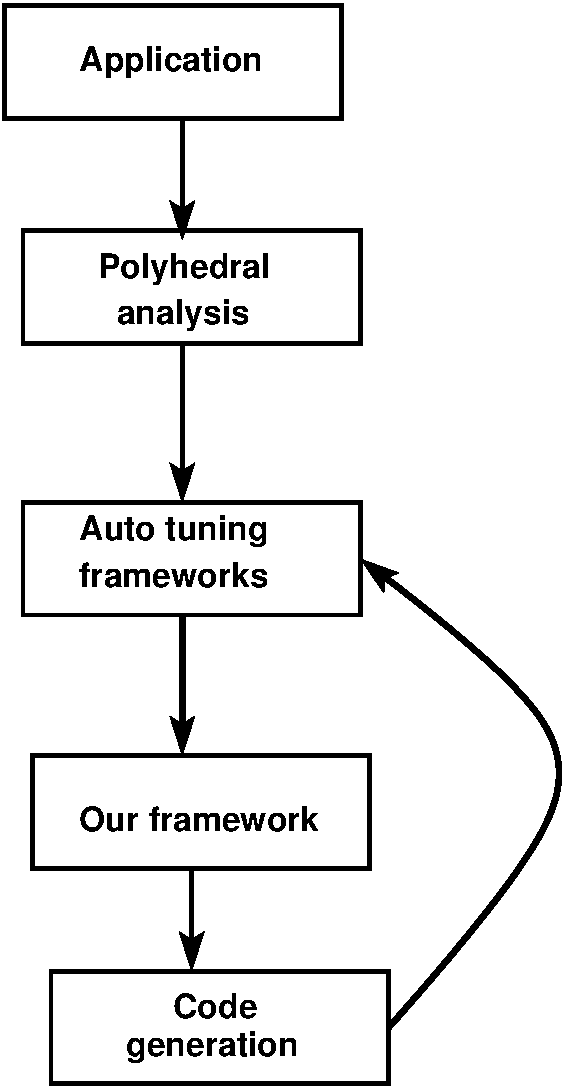
\includegraphics[scale=0.3]{./figures/tool_chain}
    \label{fig:5a}
    % \scalebox{0.4}{\input{./figures/jacobi.pdf_t}}
  }
  \subfigure[The task graph for the Jacobi example]{
    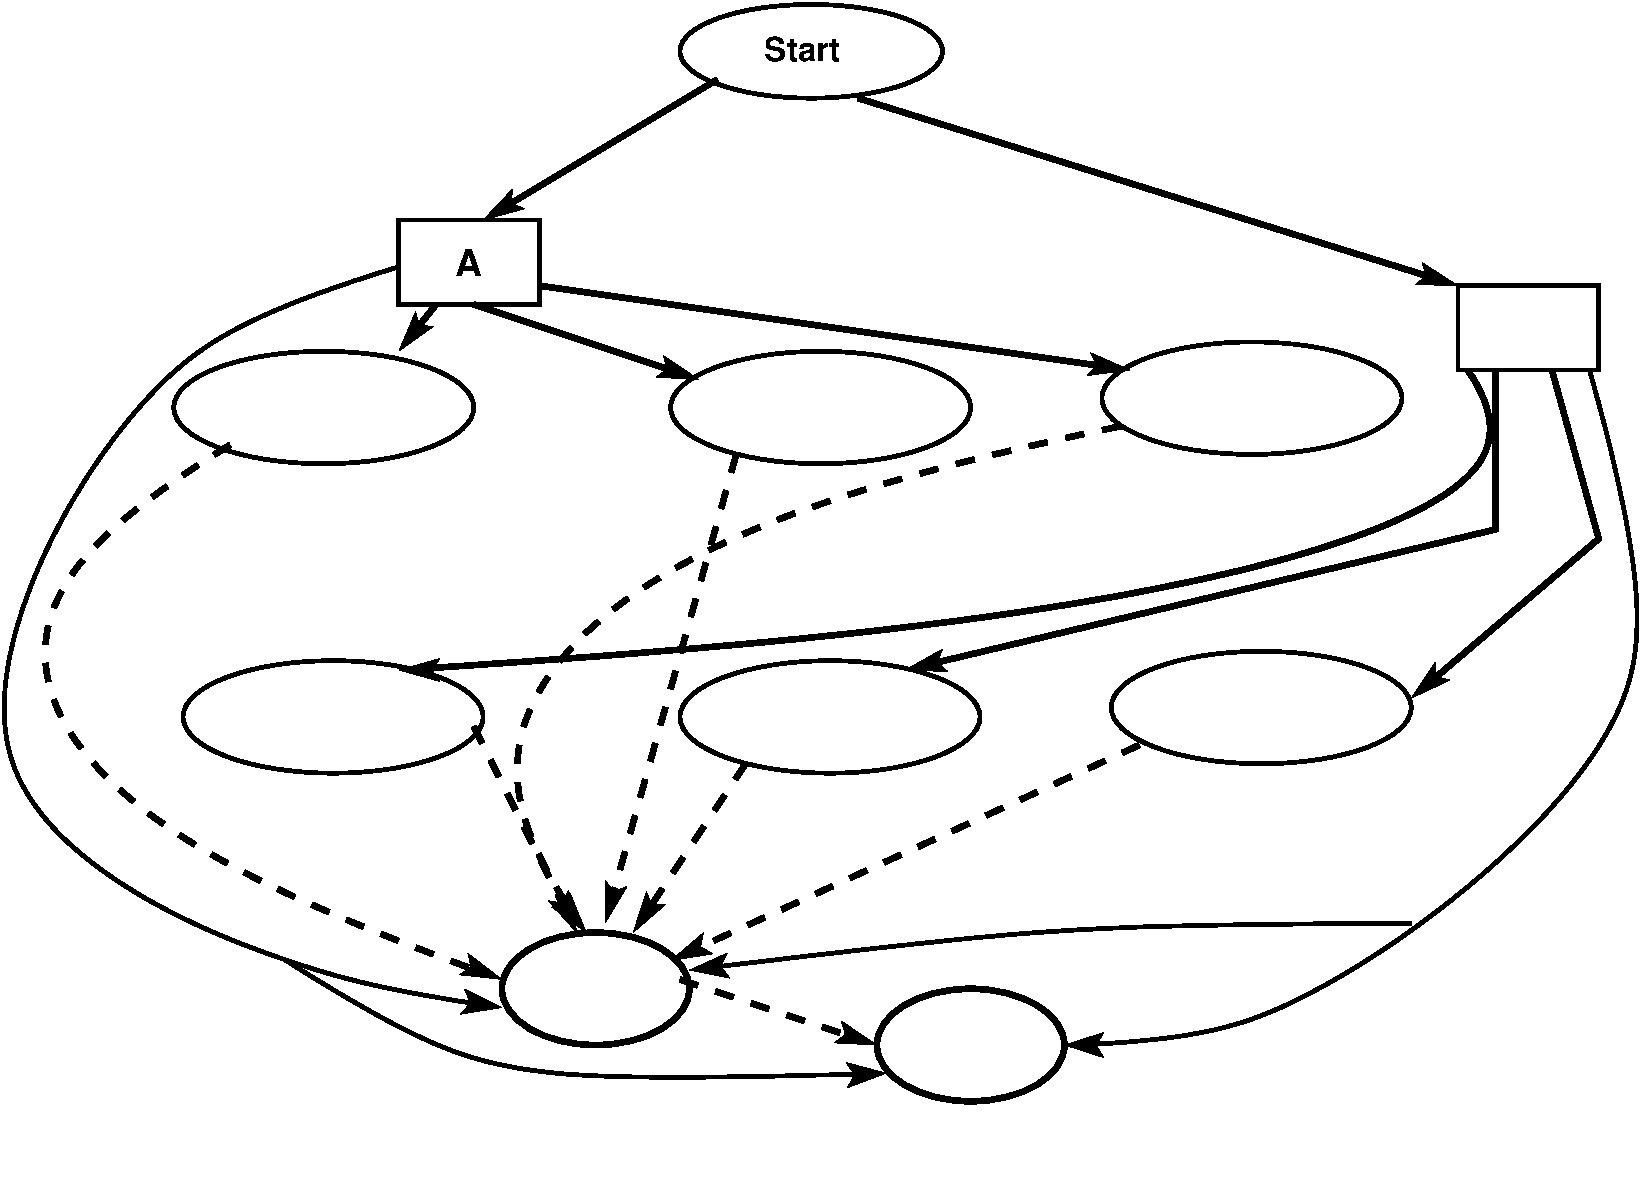
\includegraphics[scale=0.4]{./figures/jacobi}
    \label{fig:5b}
  }
  \caption{}
  \label{fig:5}
\end{figure*}

In this section we use the very popular Jacobi~\cite{jacobi2} stencil
computation to describe how our framework extracts a task graph from the
application for partitioning onto the underlying architecture. Jacobi is
an important stencil computation used in a plethora of domains such as
fluid dynamic and hence, it is worth investigating performance
improvements for Jacobi.

In Figure~\ref{fig:4}, statements \texttt{S1} and \texttt{S2} initialize
2D Jacobi matrices. Next, the actual stencil computation is carried out
in statement \texttt{S3}, for \texttt{TSTEPS} iterations. Finally,
statement \texttt{S4}, transfers the calculated data from matrix
\texttt{B} to \texttt{A}.

\begin{scriptsize}
  \begin{figure}[h!]
    \centering
\begin{verbatim}
 //Task and data-parallel
 for (int i=0;i<M; ++i){
  for (int j=0;j<N; ++j){
   S1: A[i][j] = (i*j+4.0/N)
   S2: B[i][j] = (i*j+9.0/N)
  }
 }
 for (int k=0;k<TSTEPS;++k){
  for (int i=1; i<M; ++i)
   for (int j=1; j<N; ++j)
    S3: B[i][j] = 0.2*(A[i][j]+A[i][j-1]
              +A[i][j+1]+A[i-1][j])

  //Data-parallel
  for (int i=1; i<M; ++i)
   for (int j=1; j<N; ++j)
    S4: A[i][j] = B[i][j]
 }
\end{verbatim}
    \caption{Example 2-dimensional Jacobi stencil computation}
    \label{fig:4}
  \end{figure}
\end{scriptsize}

The task graph for the 2D Jacobi stencil computation is shown in
Figure~\ref{fig:5b}. The initialization phase of the Jacobi example
consist of both task and data parallelism. In Figure~\ref{fig:5b}, the
first and second row of statements \texttt{S1\_1} to \texttt{S1\_m} and
\texttt{S2\_1} to \texttt{S2\_m}, show various loop tiles that are
generated for execution onto different processors for statements
\texttt{S1} and \texttt{S2}, respectively. Everyone of these nodes
indicate vector computations. Sample vector code within anyone of these
assignment nodes when assigned to an Intel SSE3 unit is shown in
Figure~\ref{fig:6}. Similar vector code is generated in the ptx format
for GPU allocations. We keep a count of the number of instructions for
each of these nodes. There are two counts: (1) the number of
instructions a node needs to execute iteratively. For example, node
\texttt{S3} (representing statement \texttt{S3} in the Jacobi example)
needs to iterate 998001000 times for a 1000 $\times$ 1000 matrix with
\texttt{TSTEPS} itself set to a 1000, provided it is not vectorized as
shown in Figure~\ref{fig:5b}. (2) Nodes \texttt{S1\_1} to \texttt{S1\_m} and
\texttt{S2\_1} to \texttt{S2\_m} only need to be executed once, but have
a large vector count.

Each ellipse in the task-graph is connected to a store. Stores are
represented as boxes in the task-graph. Stores have their instruction
count and vector length count set to 0. Every statement deepening upon
its vector length requires different amount of data to carry out the
computation. This data needs to be transfered from the store (the main
memory in most cases) to the caches where the task nodes are going to be
executed. We represent the about of data to be transfered in the
task-graph in bits. For example, node \texttt{S1\_1} with a smaller
vector length of 16, requires 2.2KB of data to be transfered to its
cache for computation. Node \texttt{S3} on the other hand, being
non-vectorized requires 15KB of data to be transfered to its cache.

Finally, the task graph also consists of dependence edges. In
Figure~\ref{fig:5b}, the dependence edges are marked with the dashed
lines. Dependence edges, as the name suggests show the dependence
between statements in the application. For example, statements
\texttt{S1} and \texttt{S2} are independent of each other. But,
statements \texttt{S3} and \texttt{S4} are dependent upon these
aforementioned statements. Dependence edges do not have any weights.

\begin{figure}[h!]
  \centering
\begin{verbatim}
LCPI0_0:
 .long	1018444121 ## float 2.200000e-02
 .long	1021128475 ## float 2.700000e-02
 .long	1023611503 ## float 3.200000e-02
 .long	1024953680 ## float 3.700000e-02

 movaps	LCPI0_0(%rip), %xmm8
\end{verbatim}
  \caption{Example vector code running on the Intel SSE unit}
  \label{fig:6}
\end{figure}




%%% Local Variables: 
%%% mode: latex
%%% TeX-master: "bare_conf"
%%% End: 


\section{Generating the resource graph}
\label{sec:gener-reso-graph}


\begin{figure*}[t!]
  \centering
  % \includegraphics[scale=0.42]{./figures/jacobi2d}
  \scalebox{0.45}{\section{Generating the resource graph}
\label{sec:gener-reso-graph}


\begin{figure*}[t!]
  \centering
  % \includegraphics[scale=0.42]{./figures/jacobi2d}
  \scalebox{0.45}{\section{Generating the resource graph}
\label{sec:gener-reso-graph}


\begin{figure*}[t!]
  \centering
  % \includegraphics[scale=0.42]{./figures/jacobi2d}
  \scalebox{0.45}{\input{./figures/resource_graph.pdf_t}}
  \caption{An example resource graph}
  \label{fig:1r}
\end{figure*}

We use synthetically generated graphs to test our framework, because in
a heterogeneous setup, we do not know the exact nature of the processing
elements being utilized. For example, a setup might consist of a Tesla
Nvidia GPU core connected to an Atmel micro-processor. It is also
possible that a CELL processing unit is connected to a X86 processing
element. Moreover, we cannot judge beforehand the type of bus
connections one might have on this multi-core system. In order to
overcome these issues we take a more statical view of the process. We
use synthetically generated topologies to test our framework. One such
synthetically generated resource graph is shown in Figure~\ref{fig:1r}.

In the resource graph in Figure~\ref{fig:1r}, the processing elements
are denoted via boxes. Each processing element consists of two
decorations following the previously defined formalism in
Section~\ref{sec:form-reso-graph}. In Figure~\ref{fig:1r} the processing
elements are labeled from \texttt{A} through to \texttt{P} and are
placed in a 2D tiled topology. For processing element \texttt{A} the
MIPS count is provided as $W^A_0$, while the vector length count is
provided as $W^A_1$. The bandwidth connecting the various processing
elements are denoted via $W^c$.

%%% Local Variables: 
%%% mode: latex
%%% TeX-master: "bare_conf"
%%% End: 
}
  \caption{An example resource graph}
  \label{fig:1r}
\end{figure*}

We use synthetically generated graphs to test our framework, because in
a heterogeneous setup, we do not know the exact nature of the processing
elements being utilized. For example, a setup might consist of a Tesla
Nvidia GPU core connected to an Atmel micro-processor. It is also
possible that a CELL processing unit is connected to a X86 processing
element. Moreover, we cannot judge beforehand the type of bus
connections one might have on this multi-core system. In order to
overcome these issues we take a more statical view of the process. We
use synthetically generated topologies to test our framework. One such
synthetically generated resource graph is shown in Figure~\ref{fig:1r}.

In the resource graph in Figure~\ref{fig:1r}, the processing elements
are denoted via boxes. Each processing element consists of two
decorations following the previously defined formalism in
Section~\ref{sec:form-reso-graph}. In Figure~\ref{fig:1r} the processing
elements are labeled from \texttt{A} through to \texttt{P} and are
placed in a 2D tiled topology. For processing element \texttt{A} the
MIPS count is provided as $W^A_0$, while the vector length count is
provided as $W^A_1$. The bandwidth connecting the various processing
elements are denoted via $W^c$.

%%% Local Variables: 
%%% mode: latex
%%% TeX-master: "bare_conf"
%%% End: 
}
  \caption{An example resource graph}
  \label{fig:1r}
\end{figure*}

We use synthetically generated graphs to test our framework, because in
a heterogeneous setup, we do not know the exact nature of the processing
elements being utilized. For example, a setup might consist of a Tesla
Nvidia GPU core connected to an Atmel micro-processor. It is also
possible that a CELL processing unit is connected to a X86 processing
element. Moreover, we cannot judge beforehand the type of bus
connections one might have on this multi-core system. In order to
overcome these issues we take a more statical view of the process. We
use synthetically generated topologies to test our framework. One such
synthetically generated resource graph is shown in Figure~\ref{fig:1r}.

In the resource graph in Figure~\ref{fig:1r}, the processing elements
are denoted via boxes. Each processing element consists of two
decorations following the previously defined formalism in
Section~\ref{sec:form-reso-graph}. In Figure~\ref{fig:1r} the processing
elements are labeled from \texttt{A} through to \texttt{P} and are
placed in a 2D tiled topology. For processing element \texttt{A} the
MIPS count is provided as $W^A_0$, while the vector length count is
provided as $W^A_1$. The bandwidth connecting the various processing
elements are denoted via $W^c$.

%%% Local Variables: 
%%% mode: latex
%%% TeX-master: "bare_conf"
%%% End: 


\section{Simulated annealing}
\label{sec:simulated-annealing}

Simulated Annealing~\cite{kirkpatrick} is a generic probabilistic algorithm for
finding the global optimum of a given function,
$\mathcal{F}:\mathcal{R}\rightarrow\mathcal{R}$, which has a large search space.
Simulated Annealing in most of the cases is cheaper than exhaustive enumeration,
which is exhaustively listing the entire search space. Since it is a monte carlo
method it will always terminate and the solution need not be the most optimal
but in general considered to be a good approximation of the optimum.

\subsection{Overview}

In general SA is a non-greedy heuristic algorithm which explores the search
space by moving from a higher temperature to a lower temperature. The algorithm
always accepts moves to a better solution, determined by evaluating an
\textit{objective function} and sometimes accpets moves to worse states with a
probability that changes with temperatures. Initially, when the temperature is
high, the algorithm is more tolerable and accepts moves to worse states with a
higher probability. As the temperature falls down, this probability decreases
and the alogrithm is less tolerant towards solutions with a worse value for the
objective function.

This is the reason why SA is not a purely greedy algorithm as it accepts moves
to bad states with some probability which enables it to move out of local
maximas\/minimas. But the algorithm becomes more greedier as the temperature
decreases. Figure~\ref{fig:temperature_drop} shows how the temperature drops and
how this acceptance probability changes with this drop in temperature.

\subsection{From the mapping problem standpoint}

\begin{algorithm}[1]
\caption{$Simulated\_Annealing(\zeta_0, \mathcal{T}_0)$}
\label{algo:SA}
\DontPrintSemicolon
\KwIn{Initial Mapping $\zeta_0$ and Starting Temperature $\mathcal{T}_0$}
\KwOut{Best Mapping $\zeta_{best}$}
$\zeta \leftarrow \zeta_0$ \\
$C \leftarrow OBJECTIVE\_FUNCTION(\zeta_0)$ \\
$\zeta_{best} \leftarrow \zeta$
$C_{best} \leftarrow C$
\end{algorithm}

Algorithm~\ref{algo:SA} represents the pseudocode for our algorithm. We begin by
choosing some initial starting point for our state space exploration, which from
the mapping problem standpoint is some initial mapping of tasks from $V_t$ to
PEs $V_r$. We choose our initial mapping to be all tasks from $V_t$ mapped onto
some random PE $j \in V_r$. This is a good idea because we have observed that
this puts tightly coupled tasks, i.e. tasks that communicate heavily, on the
same PE since moving them onto different PEs would incur more costs and would thus
lead to a bad state.

The \textit{OBJECTIVE\_FUNCTION} evaluates the latency of execution of the
mapping $\zeta$ on $V_r$ as described earlier in
Section~\ref{problem-definition}. $\zeta_0$ is the initial mapping chosen as
discussed in the previous paragraph, $\mathcal{T}_0$ is the starting
temperature of the annealing process and $\zeta_{current}$ and $T_{current}$ are
the current mapping and temperature respectively. $\zeta_{new}$ is the next
mapping as prescribed by the \mbox{\textit{NEXT\_STATE($\zeta_{current}$,
$T_{current}$)}} function and $\mathcal{C}_{new}$ is the cost of the new mapping
as evaluated by \textit{OBJECTIVE\_FUNCTION($\zeta_{new}$)}. $\mathcal{T}$
changes according to the \textit{NEXT\_TEMPERATURE} which is defined in the
coming section.

The \textit{NEXT\_STATE} function, which is one of the contributions of this
paper, is defined in the coming section. \textit{RAND} returns a value between
$[0, 1)$ which is then compared with the value returned by
\textit{ACCEPTANCE\_PROBABILITY}. We choose to accept a worse state based on
these two values.

\subsection{Parameter Selection}
The quality of the final solution entirely depends on the selection of values
for the parameters of interest. This configures the annealing schedule and the
acceptance probability and move functions.

We use the value for the initial and final temperature for the annealing
schedule from the paper written by Heikki et al.~\ref{parameters-SA}. 

The initial temperature $\mathcal{T}_0$ of the annealing schedule is selected as follows,
\begin{equation}
\mathcal{T}_0 = \frac{kt_{max}}{t_{minsum}}
\end{equation}
where $t_{max}$ is the maximum execution time for any task $t_i \in V_t$ on any
PE $r_j \in V_r$ and $t_{minsum}$ is the sum of execution time of all tasks $\in
V_t$ on the fastest PE $r_{fastest} \in V_r$.

The final temperature of the annealing schedule is selected as follows,
\begin{equation}
\mathcal{T}_f = \frac{t_{min}}{kt_{maxsum}}
\end{equation}
where $t_{min}$ is the minimum execution time for any task$t_i \in V_t$ on any
PE $r_j \in V_r$ and $t_{maxsum}$ is the sum of execution time of all tasks $\in
V_t$ on the slowest PE $r_{slowest} \in V_r$. In both the cases, $k$ is a
constant and $k=1$ is suitable for all our experiments.

Since the objective of this article is to map heterogeneous applications onto heterogeneous architectures, these heuristics have to be changed as well. When we  

%%% Local Variables: 
%%% mode: latex
%%% TeX-master: "bare_conf"
%%% End: 


\section{Experiments and Results}

We show the speedup obtained using our improved heuristics against the
conventional heuristics for SA as prescribed by~\cite{hors06}. We also
compare the results we obtain against the K-way graph partitioning
algorithm~\cite{gkar95} and heterogeneous bin packing
heuristic~\cite{mmar11}.

\subsection{K-way graph partitioning}
\label{sec:k-way-graph}

Graph partitioning plays an important role in the multi-processor and
VLIW scheduling and partitioning
algorithms~\cite{aale01,kpur99,enys98}. K-way graph partitioning is an
important algorithm, which partitions a given graph into K or less
parts, resulting in load balanced allocations. K-way partitioning mixed
with min-edge cuts can form a good tool to partition a task-graph onto a
multi-processor system, resulting in equal utilization of PEs and
reduced communication costs. We have utilized the Metis~\cite{gkar95}
graph partitioning tool to perform a K-way graph partitioning onto
heterogeneous multi-processor architectures for comparison purposes.

Metis is a graph partitioner, which implements K-way partitioning with
min-edge cut as the primary objective. The weights on the graph nodes
are represented as constraints. Each graph node can have multiple-node
weights representing different criteria. The edges between nodes can be
weighted themselves, but as opposed to nodes, edges can only be
decorated with a single weight. Moreover, in Metis one can use a concept
called ``tp-weights'', which give preference to different node
constraints when performing load-balancing during K-way graph
partitioning~\cite{gkar95}. % These are the only features of Metis
% that we required when implementing our algorithm. Metis provides a
% number of other features, which the readers can lookup
% in~\cite{gkar95}.

The gist of our K-way task partitioning approach onto a heterogeneous
multi-core architecture is as follows:

\begin{itemize}

\item Our resource graph is first described as a simple graph in
  Metis. In this description each of the two capabilities $W^i_0$ and
  $W^i_1$ are described as two constraints for each node in the
  graph. The communication bandwidth is described as edge weights in
  Metis.

\item Once we have the resource graph in the Metis format we calculate
  the tp-weights. There are two tp-weights generated, one for each of
  the resource node capabilities. Let us revisit the 4 $\times$ 4 mesh
  shown in Figure~\ref{fig:1r}. For each processor the MIPS tp-weight is
  calculated by the formula: $W^i_0/\sum_{\forall i \in
    V_r}(W^i_0)$. Similarly, we can easily calculate the tp-weight
  metric for each PEs vector length capability as: $W^i_1/\sum_{\forall
    i \in V_r}(W^i_1)$. These fractions give a relative approximation of
  the capabilities of each PE compared to the other. For example, given
  two nodes with $W^0_0 = 100$ and $W^1_0 = 50$, then the tp-weights for
  the first node has a tp-weight of, $0.667$, while the second has a
  tp-weight of, $0.333$.

\item The nodes in our task graph are described as graph nodes in the
  Metis format. The two requirements ($R^i_0$ and $R^i_1$) for each task
  node are described as two constraints in the Metis node format. The
  edge weights in our task graph are described as edge weights in the
  Metis graph format.

\item Once we have the task graph described in the Metis format along
  with the tp-weight metric for each PE in the resource graph. We ask
  for a $|V_r|$ partition from Metis, giving the tp-weight metric for
  each constraint of the task graph.

\item The resultant partition is then used to calculate the objective in
  Equation~(\ref{eq:2}).

\end{itemize}

\subsection{Heterogeneous bin packing heuristic}
\label{sec:heter-bin-pack}

Heuristic bin packing solutions have given good results in the general
case~\cite{ecof78}. Comparing with the heterogeneous bin packing
heuristic~\cite{mmar11} allows us to gauge the effectiveness of our
algorithm against a standard technique.

Let $\mathcal{I}$ be the items to be accommodated into the bins and let
$\mathcal{K}$ be the set of bins available.  From the standpoint of the
mapping problem, $\mathcal{I}$ refers to the set of task graph nodes
($|V_t|$) and $\mathcal{K}$ refers to the nodes in the resource graph
($|V_r|$). Similar to the Knapsack problem~\cite{sski08}, by which A-BFD
(\textit{Adaptive Best First Decreasing}) is inspired, each element $i
\in \mathcal{I},\ \mathcal{K}$ has two constraints on them represented
by $c_i$ (cost), which translates to the PE capability $W^i_0$ and $V_i$
(volume), which translates to the capability $W^i_1$, respectively.
% Right off the bat, this seems to be a significant advantage, our
% framework has over heterogeneous bin packing, as \textit{A-BFD} only
% works with two constraints whereas our framework poses no such
% restrictions.
\textit{A-BFD} proceeds to sort $\mathcal{I}$ according
to non-increasing order of their volume and sorts $\mathcal{K}$
according to non-increasing order of the ratio $c_i/V_i$. Then, it
proceeds to allocate items from $\mathcal{I}$ into best bins $b \in
\mathcal{S}$. A ``best" bin, i.e., the bin with maximum free space, is
defined as the bin volume minus the sum of volumes of the items loaded
into it. % In the mapping problem setting, this becomes a double edged
% sword as it boils down to a single constraint solving problem giving
% higher priority to the second constraint (vector requirement of the
% application-tasks $w^t_1(i)$ and vector capability of the resources
% $W^r_1(i)$).

The post pass in \textit{A-BFD} chooses every bin that has at least one
item allocated to it and tries to find an empty bin, that has a higher
or equal volume than the allocated volume on the chosen bin but also has
a lower cost. If it finds such an empty bin, then it transfers all the
items allocated to the chosen bin to the newly found empty bin which is
cheaper. One of the main advantages of \textit{A-BFD} is that it is very
fast with a best case complexity of $O(N_\mathcal{I})$ without the post
pass, where $N_\mathcal{I}$ is the number of items (number of tasks
$|V_t|$ in the application graph $G_t$). Including the post pass, the
best case complexity becomes $O(N_\mathcal{I} + N_\mathcal{K})$ where
$N_\mathcal{K}$ is the number of bins (number of PEs $|V_R|$ in the
resource graph $G_r$).

\subsection{The experimental setup}
\label{sec:experimental-setup}

We need to setup the resource graph and the task graph for experimental
purposes. Here, we describe our setup for both.

\subsubsection{The resource graph setup}
\label{sec:resource-graph-setup}

The experimental section consist of the following:

\begin{enumerate}

\item An multi-core system with \numtplgynodes nodes. A node could be
  just a multi-core CPU or a multi-core CPU with a GPU attached to
  it. \numtplgynodes varies in a normal distribution from 2 to 32.

\item The bandwidth is selected from a set \mbox{$\bwset = \{B_1, B_2, ...,
  B_{|\bwset|}\}$}. Every communication link weight ($W^c$) is selected
from the set \bwset. The elements of the set \bwset varies in the normal
distribution: 10Mb/s to 1Gb/s, representative of the multi-core
connection networks in today's machines.

\item A set of \gpunum GPUs where \gpunum is at most \numtplgynodes. The
  GPUs are connected in the network at pre-determined locations, chosen
  randomly in the normal distribution of 25\% to 75\% of $|V_r|$.

\item A set $\veclenset = \{V_1, V_2, V_3, ... V_{|\veclenset|}\}$ where
  $V_i$ is a power of 2.  Every GPU in this experiment has a vector
  length of $V_i$ where $V_i$ is sampled randomly from the set
  \veclenset. The elements of set \veclenset are chosen from a normal
  distribution ranging from 1024 to 16284.

\item A set $\corenumset = \{C_1, C_2, C_3, ... C_{|\corenumset|}\}$
  where $C_i$ is a power of 2.  Every CPU in this experiment has $C_i$
  cores where $C_i$ is sampled randomly from the set \corenumset.

\item A set $\mipsset = \{M_1, M_2, M_3, ... M_{|\mipsset|}\}$ where
  $M_i$ is a power of 2.  Every $C_i \in \corenumset$ and GPU in this
  experiment has a MIPS count of $M_i$ where $M_i$ is sampled randomly
  from the set \mipsset. The elements of set \mipsset are chosen from a
  normal distribution ranging from 100 to 1000000.

\end{enumerate}

For given values of \numtplgynodes, \gpunum, \veclenset, \corenumset,
and \mipsset and a given application, let the $k$-th \ul{trial} be
defined as one execution of the following sequence of steps.

\begin{itemize}

\item For each GPU $G_i$, sample \veclenset and \mipsset randomly to
  determine its vector length $V_i$ and MIPS count $M_i$. \label{i1}

\item For each CPU $P_i$, sample \corenumset randomly to determine the
  number of cores $C_i$ in the processor $P_i$.~\label{i2}

\item For each core $C_i$ in the processor $P_i$ sample $V_i$ and $M_i$
  randomly from set \veclenset and \mipsset.

\item Use our framework to extract data and task parallelism that is
  best utilizable by the heterogeneity created by parameters in items 1,
  2, and 3 above. Determine the execution time
  $Latency^{\zeta_\mathcal{M}}$.

\end{itemize}

An experiment, \expt(\numtplgynodes, \gpunum, \veclenset, \corenumset
\mipsset), consists of conducting enough of the above trials so that
width of the 95\% confidence interval on the average value of
$Latency^{\zeta_\mathcal{M}}$ is less than 10\% of the average
value. This results in a variable number of trials with different
experimental setups. Note that two trials differ from each other only in
the seed for the random number generator.  This reduces the dependence
of our results on a lucky sequence of numbers from the random number
generator.

\subsubsection{The task graph setup}
\label{sec:task-graph-setup}

We chose 5 applications: binomial option pricing (a financial
derivatives application), 2-dimensional convolution (for image
processing), gram Schmidt linear algebra kernel, 2-dimensional
Gauss-Seidel stencil computations, and finally our motivating example
itself the 2-dimensional Jacobi stencil computation. Next for these 5
applications, we varied the vector strip from 10 to 50, which resulted
in graphs varying from around 50 to 5000 nodes and with 23 to 12,000
edges. For example, given a task node with a vector length requirement
($w^i_1$) of 30,000 elements, a vector strip of 10 means dividing the
total vector requirement by 10, which results in 10 nodes each requiring
3000 vector elements. Similarly, the instruction count ($w^i_0$) for
each node varies depending upon the application at hand.

A detailed description of the applications and their features is shown
in Table~\ref{tab:1}. In general the vector requirement of the
applications in our benchmark suite varies from 1000 to 1 Million
elements. The instruction count varies from around 1 to 0.3 billion. The
edge weights depicting the amount of data transfer on the other hand
varies from 3000 bytes to almost 4.8 Mega byte.

\begin{table}[h!]
  \centering
  \begin{tabular}{|c|c|c|c|}
    \hline
    \textbf{Application} & \textbf{Vector strip} & $|V_t|$ & $|E_t|$ \\
    \hline
    \multirow{5}{*}{Binomial option pricing} & 10 & 82 & 206 \\
    & 20 & 102 & 306 \\
    & 30 & 122 & 406 \\
    & 40 & 142 & 506 \\
    & 50 & 162 & 606 \\
    \hline
    \multirow{5}{*}{Convolution} & 10 & 79 & 143 \\
    & 20 & 89 & 173 \\
    & 30 & 99 & 203 \\
    & 40 & 109 & 233 \\
    & 50 & 119 & 263 \\
    \hline
    \multirow{5}{*}{Gram Schmidt} & 10 & 228 & 443 \\
    & 20 & 838 & 1653 \\
    & 30 & 1848 & 3663 \\
    & 40 & 3258 & 6473 \\
    & 50 & 5068 & 10083\\
    \hline
    \multirow{5}{*}{Gauss-Seidel} & 10 & 227 & 531 \\
    & 20 & 837 & 2041 \\
    & 30 & 1847 & 4551 \\
    & 40 & 3257 & 8061 \\
    & 50 & 5067 & 12571\\
    \hline
    \multirow{5}{*}{Jacobi} & 10 & 48 & 130 \\
    & 20 & 78 & 240 \\
    & 30 & 108 & 350 \\
    & 40 & 138 & 460 \\
    & 50 & 168 & 570\\
    \hline
  \end{tabular}
  \caption{The task graph setup}
  \label{tab:1}
\end{table}

\subsection{Experimental results}
\label{sec:results}

The comparison of our simulated annealing approach with other techniques
are described in the next sub sections. In all the upcoming comparisons
we set the value of $q=0.75$ in our SA and standard SA techniques. This
value of $q$ is a good compromise between a slow running SA heuristic vs
application latencies, since a bigger value of $q$, results in larger
explored state space. For the aforementioned experimental setup our and
standard SA techniques were run for 10 minutes.

\subsubsection{Comparison with K-way partitioning}
\label{sec:comparison-with-k}

The results comparing K-way graph partitioning with our SA heuristic is
shown in Figure~\ref{fig:metis}. The 3D surface graphs shown in
Figure~\ref{fig:metis} consist of two surfaces. Each surface plots the
execution latency of the application, in $log_{10}(sec)$ scale, on the
Z-axis. The X and Y axes show the number of PEs in the underlying
architecture and the vector strip sizes, respectively.

The surface produced by the K-way partitioning heuristic is above the
surface created by our SA heuristic for most applications, other than
convolution and Jacobi. The major statistics comparing the two
approaches is provided in Table~\ref{tab:2}. In Table~\ref{tab:2}, The
\textbf{Max latency} and the \textbf{Min latency} columns, provide the
maximum and minimum application latencies observed in
Figure~\ref{fig:metis} for each of the applications. The last column
gives the \% of points in the surfaces that were better in our SA
technique compared to K-way graph partitioning.

\begin{figure*}[t!]
  \centering
  \subfigure[Binomial Option Pricing]{
    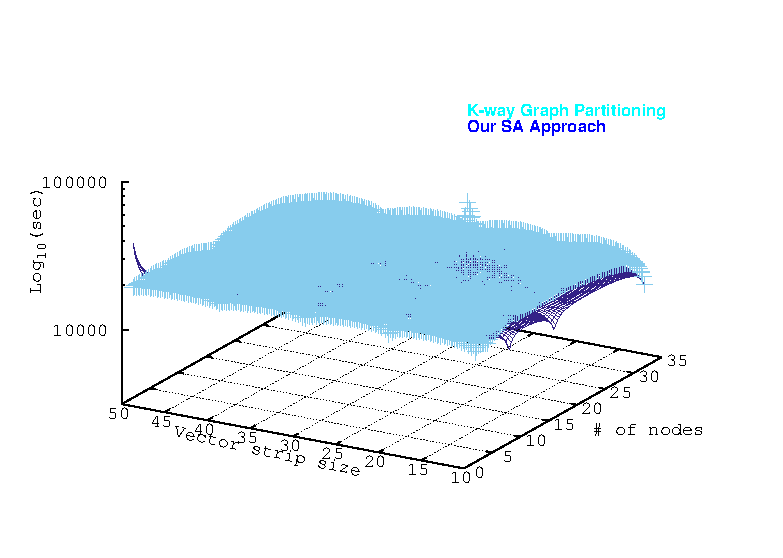
\includegraphics[angle=0, scale=0.6]{./figures/bin_metis_surface}
    \label{fig:bin1metis}
  }
  \subfigure[2 Dimensional Convolution]{
    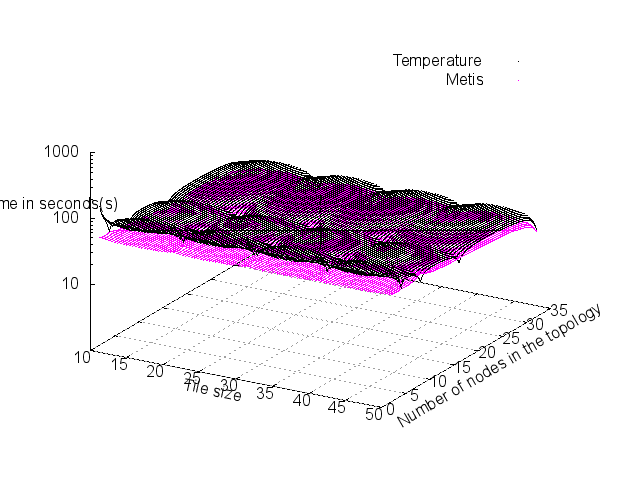
\includegraphics[angle=0, scale=0.6]{./figures/conv_metis_surface}
    \label{fig:conv1metis}
  }
  \subfigure[Gram Schmidt linear-algebra kernel]{
    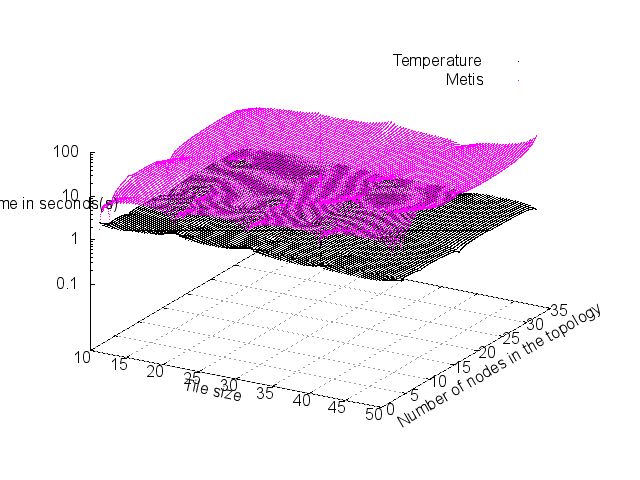
\includegraphics[angle=0, scale=0.6]{./figures/gram_metis_surface}
    \label{fig:gram1metis}
  }
  \subfigure[2 Dimensional Seidel stencil computation]{
    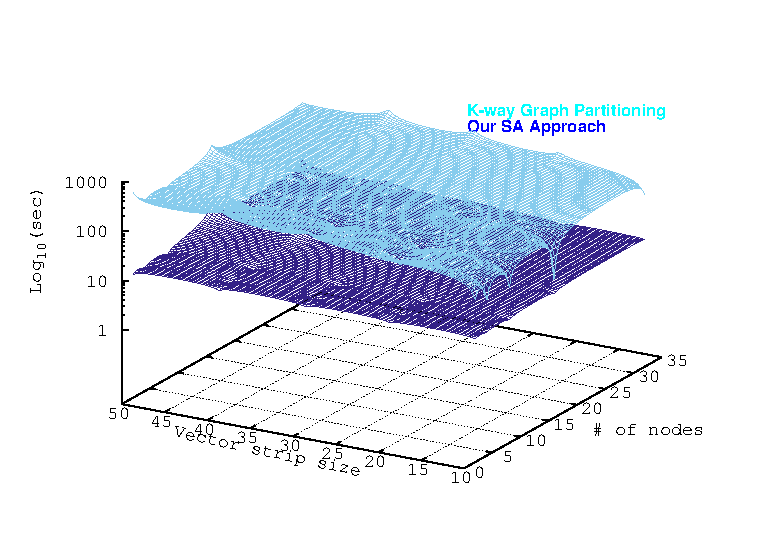
\includegraphics[angle=0, scale=0.6]{./figures/sei_metis_surface}
    \label{fig:sei1metis}
  }
  \subfigure[2 Dimensional Jacobi stencil computation]{
    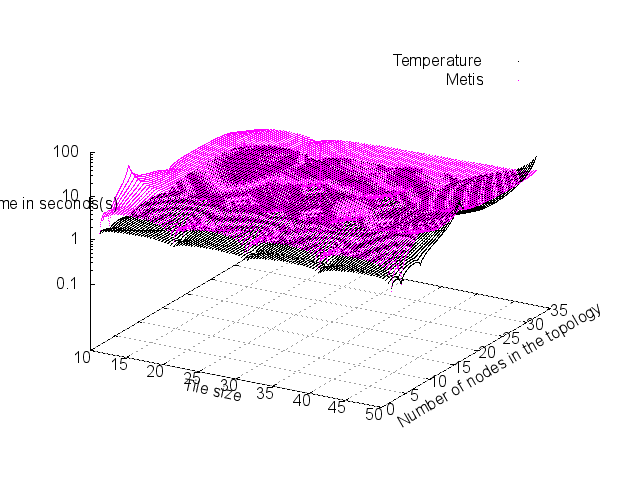
\includegraphics[angle=0, scale=0.6]{./figures/jac_metis_surface}
    \label{fig:jacl1metis}
  }
  \caption{Comparison of application latencies: Our SA approach Vs K-way
  graph partitioning (looks better in color)}
  \label{fig:metis}
\end{figure*}

\begin{figure*}[t!]
  \centering \subfigure[Major statistics comparing K-way graph
  partitioning and our SA approach for Figure~\ref{fig:metis}]{
    % \begin{table*}[t!]
      \centering
      \begin{tabular}{|c|c|c|c|c|c|}
        \hline
        \textbf{Application} &
        \multicolumn{2}{|c|}{\textbf{Max latency (sec)}} &
        \multicolumn{2}{|c|}{\textbf{Min latency (sec)}} &
        \textbf{Our SA better than K-way (\%)} \\
        \hline
        & {K-way} & {Our SA approach} &
        {K-way} & {Our SA approach} & K-way vs Our SA approach\\
        \hline
        Binomial option pricing & 79947.2 & 53404.8 & 11218.1 & 10975.5 & 94 \\
        \hline
        Convolution & 52.85 & 124.309 & 19.64 & 19.64 & 12\\
        \hline
        Gram Schmidt & 54.13 & 2.96 & 1.33 & 0.91 & 64\\
        \hline
        Gauss-Seidel & 542.44 & 32.99 & 9.67 & 9.67 & 68\\
        \hline
        Jacobi & 16 & 14.69 & 0.95 & 0.89 & 32\\
        \hline
      \end{tabular}
      % \caption{Major statistics comparing K-way graph partitioning and our
      %   SA approach}
      \label{tab:2}
    % \end{table*}
  }
  \subfigure[Major statistics comparing heterogeneous bin packing and our
      SA approach for Figure~\ref{fig:ho}]{
    % \begin{table*}[t!]
    \centering
    \begin{tabular}{|c|c|c|c|c|c|}
      \hline
      \textbf{Application} &
      \multicolumn{2}{|c|}{\textbf{Max latency (sec)}} &
      \multicolumn{2}{|c|}{\textbf{Min latency (sec)}} &
      \textbf{Our SA better than HBP (\%)} \\
      \hline
      & {HBP} & {Our SA approach} &
      {HBP} & {Our SA approach} & HBP vs Our SA approach\\
      \hline
      Convolution & 215741 & 124.309 & 98.45 & 19.64 & 92\\
      \hline
      Gram Schmidt & 3169.72 & 2.96 & 2947.65 & 0.91 & 92\\
      \hline
      Jacobi & 4653.66 & 14.69 & 1.69 & 0.89 & 92\\
      \hline
    \end{tabular}
    % \caption{}
    \label{tab:3}
    % \end{table*}
  } \subfigure[Major statistics comparing standard SA vs our SA approach
  for Figure~\ref{fig:stdsa}]{
    % \begin{table*}[t!]
    \centering
    \begin{tabular}{|c|c|c|c|c|c|}
      \hline
      \textbf{Application} &
      \multicolumn{2}{|c|}{\textbf{Max latency (sec)}} &
      \multicolumn{2}{|c|}{\textbf{Min latency (sec)}} &
      \textbf{Better (\%)} \\
      \hline
      & {Standard SA} & {Our SA} &
      {Standard SA} & {Our SA} & Standard SA vs Our SA\\
      \hline
      Binomial option pricing & 219230 & 53404.8 & 25967.5 & 8971 & 95 \\
      \hline
      Convolution & 220525 & 124.31 & 50.34 & 19.64 & 76\\
      \hline
      Gram Schmidt & 10.04 & 2.96 & 0.96 & 0.91 & 92\\
      \hline
      Gauss-Seidel & 14607.8 & 32.99 & 9.07 & 9.67 & 72\\
      \hline
      Jacobi & 3504.44 & 14.69 & 0.95 & 0.89 & 88\\
      \hline
    \end{tabular}
    % \caption{}
    \label{tab:4}
    % \end{table*}
  }
  \caption{Statistical comparisons for different benchmarks detailing
    Figures~\ref{fig:metis},~\ref{fig:ho}, and~\ref{fig:stdsa}}
  \label{fig:8}
\end{figure*}

\subsubsection{Comparison with heterogeneous bin packing heuristic}
\label{sec:comp-with-heter}

Comparison of our SA technique with heterogeneous bin packing heuristic
is shown in Figure~\ref{fig:ho}. Unlike, K-way graph partitioning, the
bin packing heuristic could not partition the binomial option pricing
and Gauss-Seidel examples for any vector strip size, because the bin
packing algorithm gives up if there is no underlying PE that can support
the required vector tile size. Our SA heuristic on the other hand runs a
part of the vector on the underlying PE and then iterates in a loop
until all vector computations are finished. For example, if the task
graph requires a 1000 vector elements that need to be processed at once,
and the largest vector capability in the resource graph is a 100, then,
our heuristic will allocate a 100 vector elements onto the underlying
hardware and then increase the instruction count by 10.

The heterogeneous bin packing heuristic performs much worse compared to
our approach. This can be blamed onto the fact that heterogeneous bin
packing prioritizes vector length over number of instruction
count. Heterogeneous bin packing packs a large number of vectors nodes
from the application graph into a single large vector PE, including
those task nodes, which have a very small vector count ($w^i_0$), but a
very large instruction count ($w^i_1$). The major facts about
Figure~\ref{fig:ho} are highlighted in Table~\ref{tab:3}.

\begin{figure*}[t!]
  % \centering
  \subfigure[2 Dimensional Convolution]{
    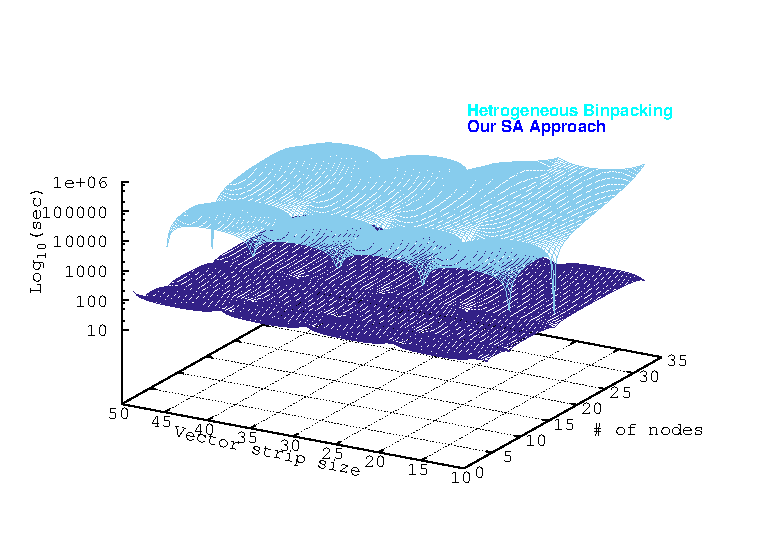
\includegraphics[angle=0, scale=0.6]{./figures/conv_hbp_surface}
    \label{fig:conv1ho}
  }
  \subfigure[Gram Schmidt linear-algebra kernel]{
    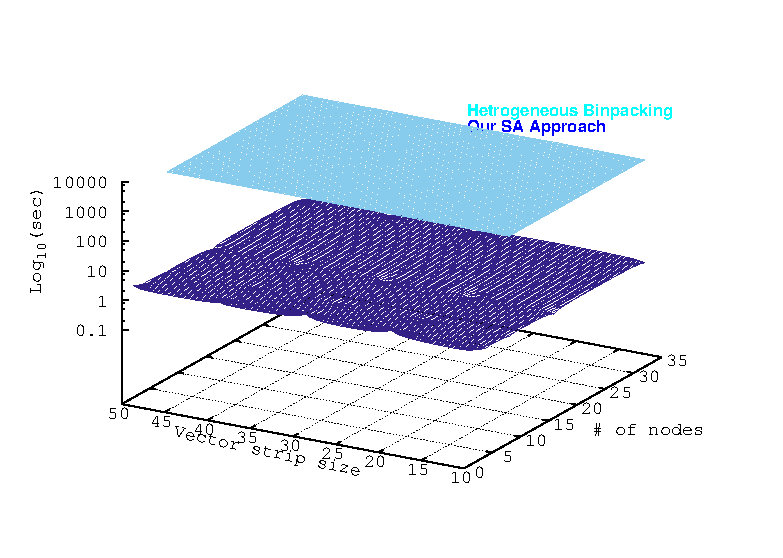
\includegraphics[angle=0, scale=0.6]{./figures/gram_hbp_surface}
    \label{fig:gram1ho}
  }
  \subfigure[2 Dimensional Jacobi stencil computation]{
    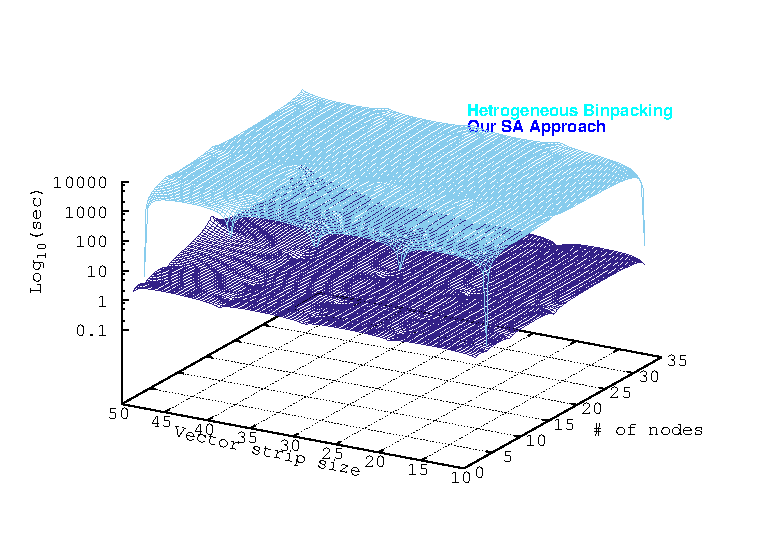
\includegraphics[angle=0, scale=0.6]{./figures/jac_hbp_surface}
    \label{fig:jacl1ho}
  }
  \caption{Comparison of execution times of ``Our SA technique" and
    ``Heterogeneous Bin Packing" (looks better in color)}
  \label{fig:ho}
\end{figure*}


\subsubsection{Comparison with established SA}
\label{sec:comp-with-establ}

The figures showing the comparison of our approach with the established
SA approach of~\cite{hors06} as shown in Figure~\ref{fig:stdsa}. There
is not a single case where our SA approach is worse than the current
established technique. The major statistics comparing the two techniques
for Figure~\ref{fig:stdsa} are shown in Table~\ref{tab:4}.

The reasons for this are two fold,
\begin{itemize}
\item We change the annealing schedule such that the search exploration is
global initially, i.e. high temperatures, and it becomes local to the current
best solution as temperature drops.
\item We also get a better result because we do not permit multiple mapping
iterations per temperature level which prevents a higher percentage of tasks
moving to random PEs. 
\end{itemize}

% In all the figures and statistics presented, we ran the conventional SA and our
% improved SA approach with a maximum time limit of 10 minutes, i.e. SA will
% terminate after 10 minutes if it has not already found a solution it is
% satisfied with. The experiments were performed on a quad-core dual processor
% system with 24 gigabytes of RAM.

\begin{figure*}[h!]
  \centering
  \subfigure[Binomial Option Pricing]{
    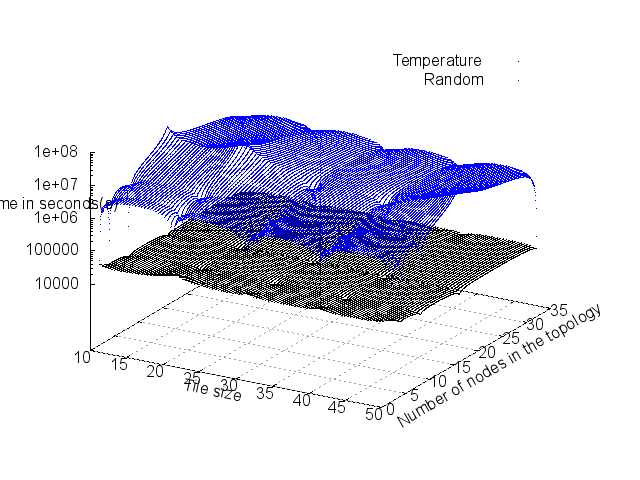
\includegraphics[angle=0, scale=0.67]{./figures/bin_random_surface}
    \label{fig:bin1random}
  }
  \subfigure[2 Dimensional Convolution]{
    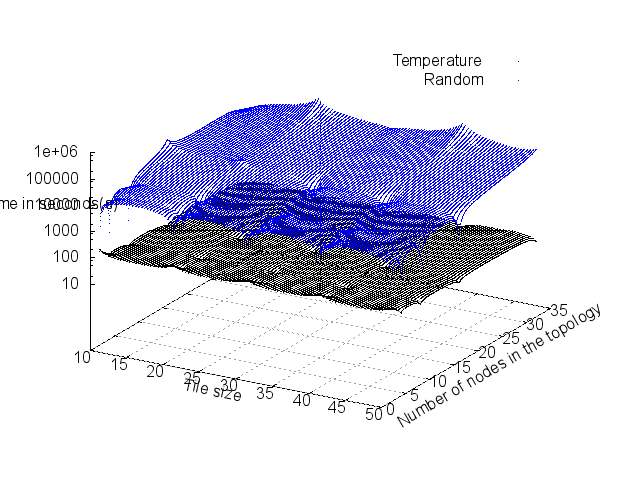
\includegraphics[angle=0, scale=0.67]{./figures/conv_random_surface}
    \label{fig:conv1random}
  }
  \subfigure[Gram Schmidt linear-algebra kernel]{
    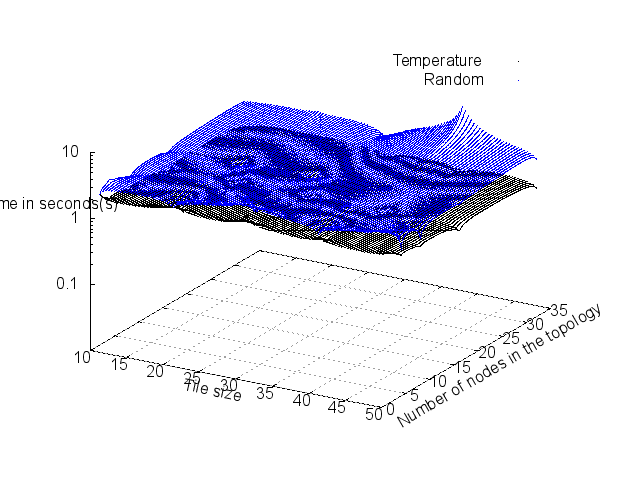
\includegraphics[angle=0, scale=0.67]{./figures/gram_random_surface}
    \label{fig:gram1random}
  }
  \subfigure[2 Dimensional Seidel stencil computation]{
    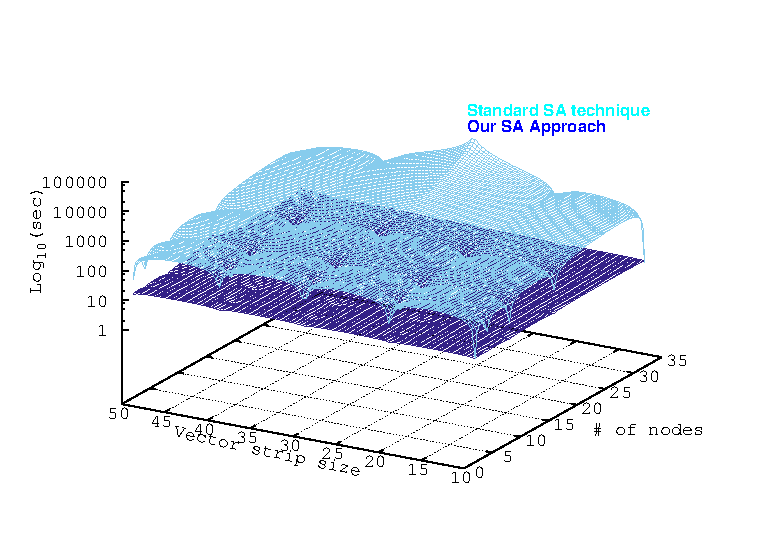
\includegraphics[angle=0, scale=0.67]{./figures/sei_random_surface}
    \label{fig:sei1random}
  }
  \subfigure[2 Dimensional Jacobi stencil computation]{
    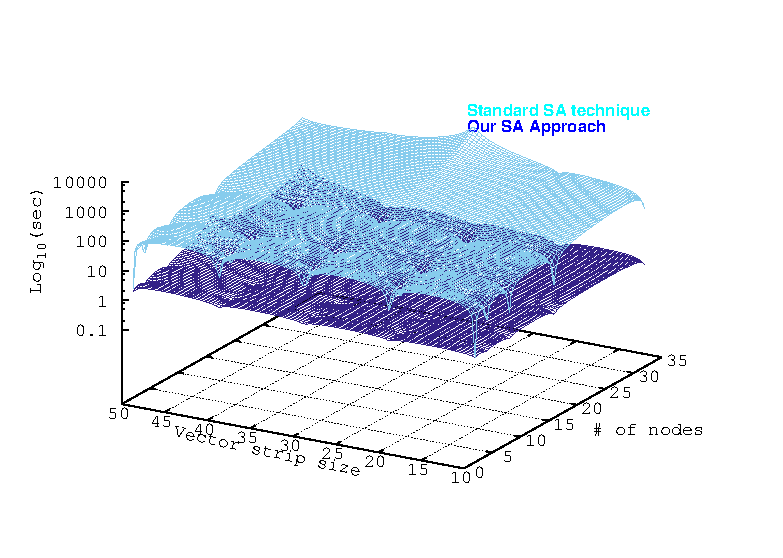
\includegraphics[angle=0, scale=0.67]{./figures/jac_random_surface}
    \label{fig:jacl1random}
  }
  \caption{Comparison of application latencies: Our SA approach vs
    standard SA approach (looks better in color)}
  \label{fig:stdsa}
\end{figure*}

% \subsubsection{Effect of varying temperature}
% \label{sec:varying-temperature}


%%% Local Variables: 
%%% mode: latex
%%% TeX-master: "bare_conf"
%%% End: 


\section{Conclusion}


% \section*{Acknowledgment}


% The authors would like to thank...
% more thanks here


\scriptsize{
\bibliographystyle{IEEEtran}
% \bibliography{latex8}
\bibliography{/Users/amal029/Dropbox/BIBLIOGRAPHY_DATABASE/main_bib.bib}
}

% that's all folks
\end{document}



%%% Local Variables: 
%%% mode: latex
%%% TeX-master: t
%%% End: 
